%%%%%%%%%%%%%%%%%%%%%%%%%%%%%%%%%%%%%%%%%%%%%%%%%%%%%%%%%%%%%%%%%%%%%%%%%%%%%%%%
\documentclass[presentation]{beamer} %\mode<presentation>{\usetheme{sapere}}
\usetheme{CambridgeUS}
\usecolortheme{orchid}

\definecolor{themeColor}{HTML}{295D98}

\setbeamercolor*{structure}{bg=black,fg=themeColor}

\setbeamercolor*{palette primary}{use=structure,fg=white,bg=structure.fg}
\setbeamercolor*{palette secondary}{use=structure,fg=white,bg=structure.fg!75}
\setbeamercolor*{palette tertiary}{use=structure,fg=white,bg=structure.fg!50!black}
\setbeamercolor*{palette quaternary}{fg=white,bg=black}

\setbeamercolor{section in toc}{fg=black,bg=white}
\setbeamercolor{alerted text}{use=structure,fg=structure.fg!50!black!80!black}

\setbeamercolor{titlelike}{parent=palette primary,fg=structure.fg!50!black}
\setbeamercolor{frametitle}{bg=structure.fg!10!white,fg=structure.fg!50!black!80!black}

\setbeamercolor*{titlelike}{parent=palette primary}


\usepackage[utf8]{inputenc}
\usepackage{amssymb}
\usepackage{graphicx}
\usepackage{subfigure}
\usepackage{multirow}
\usepackage{hhline}
\usepackage{amsfonts,amstext,amssymb,wasysym}
\usepackage{fancyvrb}
\usepackage{alltt}
\usepackage{textcomp}
\usepackage{url}
\usepackage{multimedia,pgf}
\usepackage{geometry}
\usepackage{listings}
\usepackage{framed}
\usepackage{cleveref}

\definecolor{Fuchsia}{HTML}{8C368C}
\definecolor{OliveGreen}{HTML}{3C8031}

% Code highlighting
\newcommand{\il}[1]{{\it \textcolor{gray}{// #1}}} % inline comment
\newcommand{\km}[1]{\textcolor{purple}{#1}} % key mechanism primitives
\newcommand{\ex}[1]{\textcolor{blue}{#1}} % external imported Java values
\newcommand{\fc}[1]{\textcolor{Fuchsia}{#1}} % field calculus calls
\newcommand{\fn}[1]{\textcolor{blue}{#1}} % building block / function calls
\newcommand{\vb}[1]{\textcolor{OliveGreen}{#1}} % variables
\newcommand{\str}[1]{\textcolor{darkgray}{#1}} % strings

\newcommand{\bral}{\textrm{{\tt {\char '173}}}\,}
\newcommand{\brar}{\textrm{{\tt {\char '175}}}}
\newcommand{\var}{\texttt{x}}
\newcommand{\asgK}{~\texttt{=}~}
\newcommand{\letK}{\texttt{let}~}
\newcommand{\tupK}[1]{\texttt{[}#1\texttt{]}}
\newcommand{\lambdaK}[2]{\texttt{(}#1\texttt{)->}#2}
\newcommand{\bodyK}[1]{\bral\! #1\!\brar}
\newcommand{\dotK}{\texttt{.}}
\newcommand{\applyK}{\texttt{apply}}
\newcommand{\mname}{\ex{\texttt{m}}}
\newcommand{\aname}{\ex{\texttt{\#a}}}
\newcommand{\repK}[3]{\texttt{\fc{rep}(#1<-#2)}#3}
\newcommand{\ifK}[3]{\texttt{\fc{if}}(#1)#2\,\texttt{\fc{else}}\,#3}
\newcommand{\muxK}[3]{\texttt{\fc{mux}}(#1)#2\,\texttt{\fc{else}}\,#3}
\newcommand{\nbrK}[1]{\texttt{\fc{nbr}}#1}

\title[Protelis --- Aggregate programming]{Protelis: Practical Aggregate Programming}

\author[Pianini, Viroli, Beal]
{
\parbox[b][0.3cm][c]{0.5\textwidth}{
\textbf{Danilo Pianini}, Mirko Viroli
\\
{\footnotesize \{\textbf{danilo.pianini},mirko.viroli\}\textbf{@unibo.it}}
}
\parbox[b][0.3cm][c]{0.3\textwidth}{
Jacob Beal
\\
\footnotesize jakebeal@bbn.com}
}

\institute[UniBo / BBN]
{
\parbox[t][1.5cm][c]{0.45\textwidth}{
\begin{center}
Universit\`a di Bologna
\\ Italy
\end{center}
}
\parbox[t][1.5cm][c]{0.4\textwidth}{
\begin{center}
Raytheon BBN Technologies
\\ United States of America
\end{center}
}
}

\AtBeginSection[]
{
  \begin{frame}<beamer>
    \frametitle{Outline}
    \tableofcontents[currentsection]
  \end{frame}
}

\date[2015-04-16 SAC/CM]{Symposium on Applied Computing 2015 \\ Salamanca}


\pgfdeclareimage[height=0.625cm]{university-logo}{imgs/logo}
\logo{\pgfuseimage{university-logo}}


\begin{document}


%===============================================================================
\frame[label=coverpage]{\titlepage}
%===============================================================================

\section*{Outline}
\subsection*{You'll soon have your God, and you'll make it with your hands.}
%===============================================================================
\frame{\tableofcontents}

\section{Aggregate Programming}

\subsection{Local to Global}

\begin{frame}{Our stage}

\begin{block}{}
  \begin{itemize}
    \item Large number of devices or services
    \item Possibly situated
    \item Capable of sensing, computing, communicating
    \item Behaviour must be coordinated to achieve a global goal
    \item Pervasive Continuum or (pick the one you prefer):
    \begin{itemize}
      \item Pervasive computing
      \item Smart cities
      \item Internet of things
    \end{itemize}
  \end{itemize}
\end{block}
\end{frame}

\begin{frame}{Classic approach}
\begin{block}{Local to global}
  \begin{itemize}
    \item Complex global behaviour
    \item Simple local behaviour
    \item The whole is more than the sum of the parts
    \item Interaction is key
  \end{itemize}
\end{block}
\begin{block}{Nature inspiration}
   Several systems use nature as inspiration:
  \begin{itemize}
    \item physical particles \cite{mamei2009acm}
    \item chemical reactions \cite{sapere-procedia7}
    \item ants, termites and other social insects \cite{swarmlinda}
    \item Very brief list! There are many more.
  \end{itemize}
\end{block}
\end{frame}

\begin{frame}{Nice properties and hard challenges}
  \begin{block}{The beauty}
    \begin{itemize}
      \item High resilience and fault tolerance
      \item Self adaptation
      \item Openness
      \item Self healing
    \end{itemize}
  \end{block}
  \begin{block}{The beast}
    Local to global is hard to engineer
    \begin{itemize}
      \item The desired functionality happens at the aggregate level
      \item It is very difficult to design the local behaviour in such a way that the interaction of many of them produces the desired global behaviour
      \item Many attempts, but no good engineering processes to safely design such systems
      \item Often, development becomes a try-and-simulate loop
    \end{itemize}
  \end{block}
\end{frame}

\begin{frame}{Collective to local}
   \begin{center}
      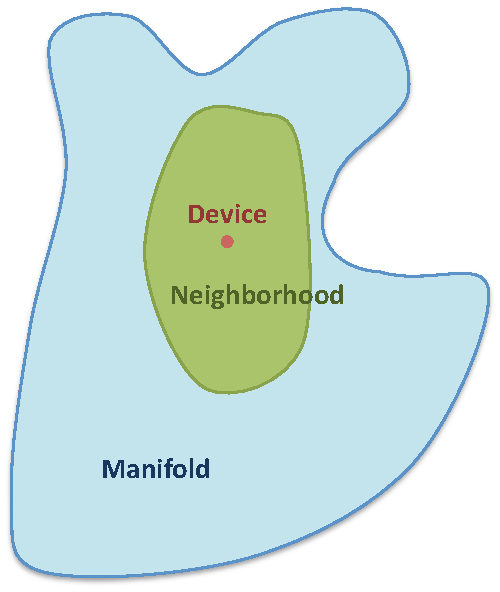
\includegraphics[width=.3\textwidth{}]{imgs/space-continuous}
      \hspace{1cm}
      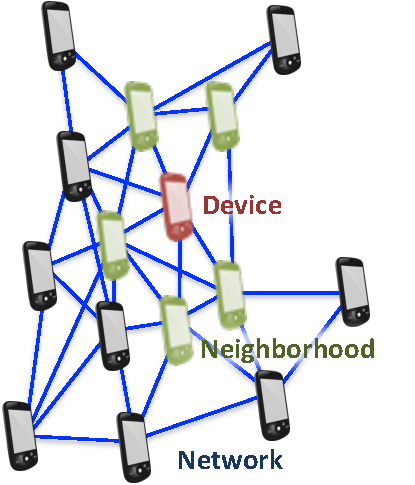
\includegraphics[width=.3\textwidth{}]{imgs/space-discrete}
   \end{center}
%   \begin{block}{Desiderata}
%     \begin{itemize}
%       \item We want to achieve a collective behaviour
%       \item We want to move our focus and abstractions towards the \emph{the whole network}, rather than focussing on the single devices that compose it and their interaction
%       \item We want to support space-time abstractions
%     \end{itemize}
%   \end{block}
  \begin{block}{Possible solution}
    \begin{itemize}
      \item Create a language that allows to express collective properties
      \item Create a runtime that can run such programs
      \begin{itemize}
         \item Possibly, also create a tool to test programs prior to deployment
      \end{itemize}
    \end{itemize}
  \end{block}
\end{frame}

\subsection{From Proto to Field Calculus}

\begin{frame}[fragile]{Existing languages}
  \begin{block} {MIT Proto \cite{proto} is the most known and successful}
   \begin{itemize}
    \item Developed at MIT and maintained at BBN Technologies
    \item Functional language, LISP-like syntax (I know you hate it too)
    \item \emph{All devices run the same program}
    \item Computation happens in rounds:
    \begin{itemize}
      \item Every device sleeps for some time
      \item Processes the messages received from the neighbours
      \item Executes its program
      \item Sends all the neighbours its result
    \end{itemize}
    \item Complex operational semantics
    \item Difficult to maintain and extend 
   \end{itemize}
  \end{block}
\end{frame}

\begin{frame}[fragile]{Field Calculus}
  \begin{block} {A ``distillate'' of Proto}
   \begin{itemize}
    \item Provides a lightweight operational semantics \cite{VDB-FOCLASA-CIC2013}
    \item ((((LISP-like syntax))))
    \item Still a functional language
    \item Simple enough to formally prove properties, powerful enough to be universal (proved!)
    \item Theoretical object, no runtime nor simulation tool provided
   \end{itemize}
  \end{block}
%   \begin{block} {Key mechanism: alignment}
%    \begin{itemize}
%     \item At the end of each cycle, send to your neighbours your annotated AST
%     \item At the beginning of each cycle, each device can inspect what was happening in its surroundings
%     \item If two devices took different branches of a \texttt{if}, they are no longer aligned until such branch returns
%    \end{itemize}
%   \end{block}
\end{frame}


\section{Protelis}

\subsection{Language features}

\begin{frame}{Ordinary language features}
  \begin{block} {}
   \begin{itemize}
    \item Functional language
    \item Same operational semantics of the field calculus 
    \item C-family syntax with infix operators
    \item Java interoperability: static methods imports and calls, method invocation with dynamic binding
    \item Higher order functions (functions as arguments, lambdas)
    \item Dynamic code
   \end{itemize}
  \end{block}
\end{frame}

\begin{frame}{Field calculus operators}
  \begin{block} {\texttt{rep}}
   \begin{itemize}
    \item defines a locally visible variable
    \item Retains its value at each computation round
    \item Enables stateful computation
   \end{itemize}
  \end{block}
  \begin{block} {\texttt{nbr}}
   \begin{itemize}
    \item Builds a field
    \begin{itemize}
      \item Map device \textrightarrow value
      \item Includes self
    \end{itemize}
    \item \texttt{*hood} built-in functions summarize the field back to ordinary expressions
   \end{itemize}
  \end{block}
\end{frame}

\begin{frame}{Branching}
  \begin{block} {\texttt{mux / else}}
   \begin{itemize}
    \item Functional inclusive ``multiplexing'' branching
    \item Evaluates both branches, then returns the correct one
    \item \texttt{nbr}s in branches can ``align''
   \end{itemize}
  \end{block}
  \begin{block} {\texttt{if / else}}
   \begin{itemize}
    \item Exclusive branching: \texttt{nbr}s in different branches do not ``align''
    \item Network gets partitioned into two regions
   \end{itemize}
  \end{block}
\end{frame}

\begin{frame}[fragile]{Code example}
\begin{Verbatim}[fontsize=\scriptsize, frame=single, commandchars=\\\{\}]
\km{def} \fn{count}() \{
   \repK{\vb{\var}}{0} {\bodyK{\vb{\var} + 1\; } }
\}

\km{def} \fn{maxh}(\vb{field}) \{ \fc{maxHood}(\nbrK{\{\vb{field}\}}) \}

\km{def} \fn{distanceTo}(\vb{source}) \{
   \fc{rep} (\vb{d} <- \fc{Infinity}) \{
      \fc{mux} (\vb{source}) \{ 0 \} \fc{else} \{ \fc{minHood}(\fc{nbr}\{\vb{d}\} + \fc{nbrRange}) \}
   \}
\}

\km{def} \fn{distanceToWithObstacle}(\vb{source}, \vb{obstacle}) \{
   \fc{if} (\vb{obstacle}) \{ \fc{Infinity} \} \fc{else} \{ \fn{distanceTo}(\vb{source}) \}
\}
\end{Verbatim}
\end{frame}

\subsection{Simulator and Runtime}

\begin{frame}{Architecture}
  \begin{block} {Implementation, distribution}
   \begin{itemize}
    \item Based on Xtext
    \item Eclipse plugin
    \item Integrated with Alchemist \cite{alchemist-jos2013}
    \item Stand-alone framework for real devices
    \item Write once, run everywhere --- evolved :)
    \item Now distributed through Maven Central \footnote{artifact: \texttt{it.unibo.alchemist:alchemist.protelis}}
   \end{itemize}
  \end{block}
\end{frame}

\begin{frame}{Abstract architecture}
  \centering
  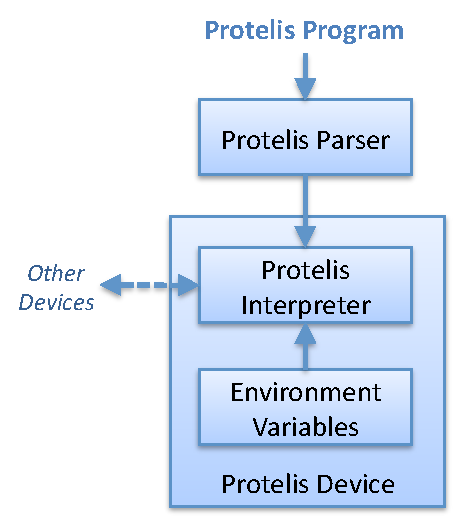
\includegraphics[height=0.8\textheight{}]{imgs/abstract}
\end{frame}

\begin{frame}{Simulation runtime architecture}
  \centering
  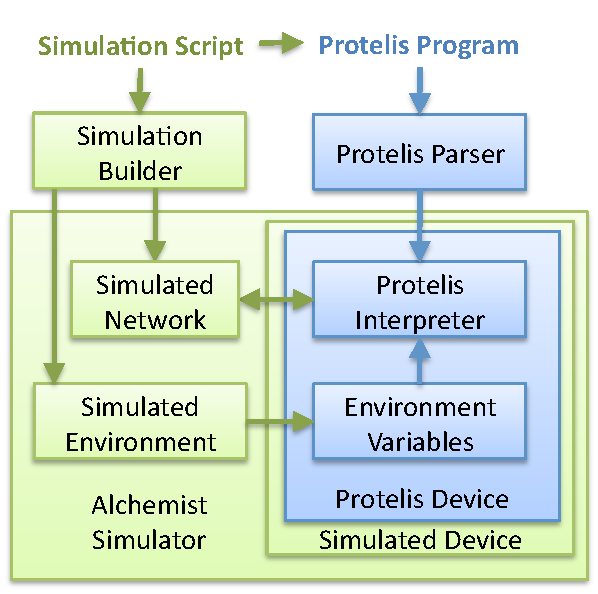
\includegraphics[width=0.6\textwidth{}]{imgs/simulated}
\end{frame}

\begin{frame}{Standalone runtime architecture}
  \centering
  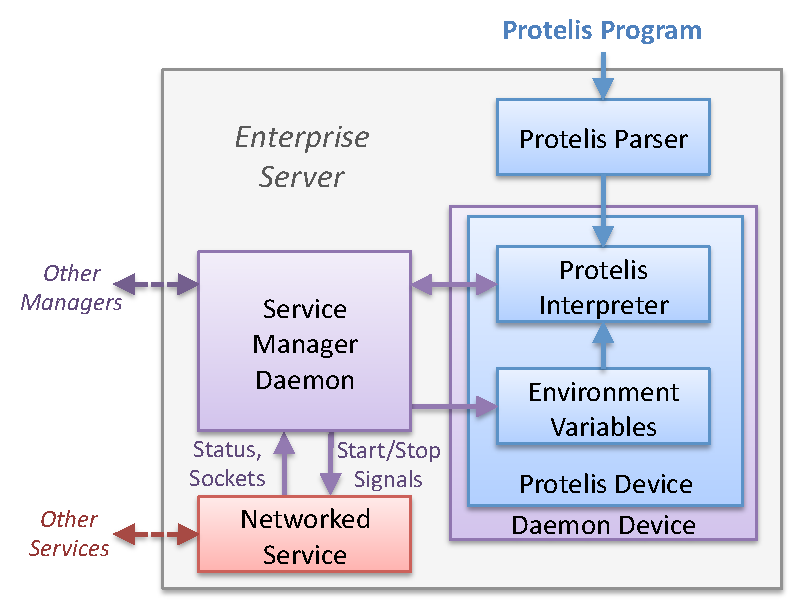
\includegraphics[width=0.8\textwidth{}]{imgs/embedded}
\end{frame}

\subsection{Examples}

\begin{frame}{Rendezvous at a Mass Event}
  \begin{block} {Problem}
   \begin{itemize}
    \item Large public event
    \item People want to rendezvous with a companion
    \item Cloud-based services may be unreachable
   \end{itemize}
  \end{block}
  \begin{block} {Possible solution with Protelis}
   \begin{itemize}
    \item Simple P2P geometric calculation across network
   \end{itemize}
  \end{block}
  \begin{block} {Testbed}
   \begin{itemize}
    \item Simulated in Alchemist
   \end{itemize}
  \end{block}
\end{frame}

\begin{frame}{Rendezvous at a Mass Event}
  \centering
  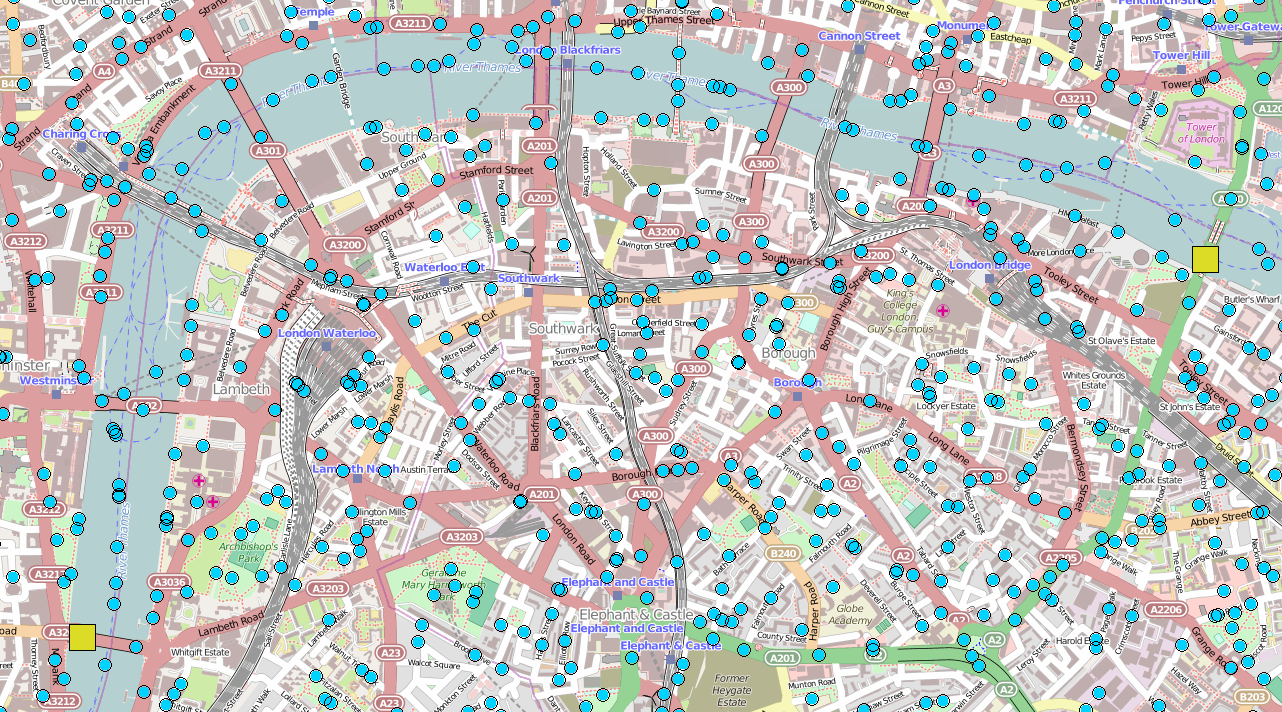
\includegraphics[width=\textwidth{}]{imgs/screenshots/london0}
\end{frame}

\begin{frame}[fragile]{Rendezvous at a Mass Event}
\begin{Verbatim}[fontsize=\scriptsize, frame=single, commandchars=\\\{\}]
\il{Follow the gradient of a potential field down from a source}
\km{def} \fn{descend}(\vb{source}, \vb{potential}) \{
  \fc{rep}(\vb{path} <- \vb{source}) \{
    \km{let} \vb{nextStep} \km{=} \fc{minHood}(\fc{nbr}([\vb{potential}, \fc{self}.\ex{getId}()]));
    \fc{if} (\vb{nextStep}.\ex{size}() > 1) \{
      \km{let} \vb{candidates} = \fc{nbr}([\vb{nextStep}.\ex{get}(1), \vb{path}]);
      \vb{source} || \fc{anyHood}([\fc{self}.\ex{getId}(), true] == \vb{candidates})
    \} \fc{else} \{
      \vb{source}
    \}
  \}
\}
\km{def} \fn{rendezvous}(\vb{person1}, \vb{person2}) \{
  \fn{descend} (\vb{person1} == \vb{owner}, \fn{distanceTo}(\vb{person2} == \vb{owner}))
\}
\il{Example of using rendezvous}
\fn{rendezvous}(\str{"Alice"}, \str{"Bob"});
\end{Verbatim}
\end{frame}

\begin{frame}{Rendezvous at a Mass Event}
  \centering
  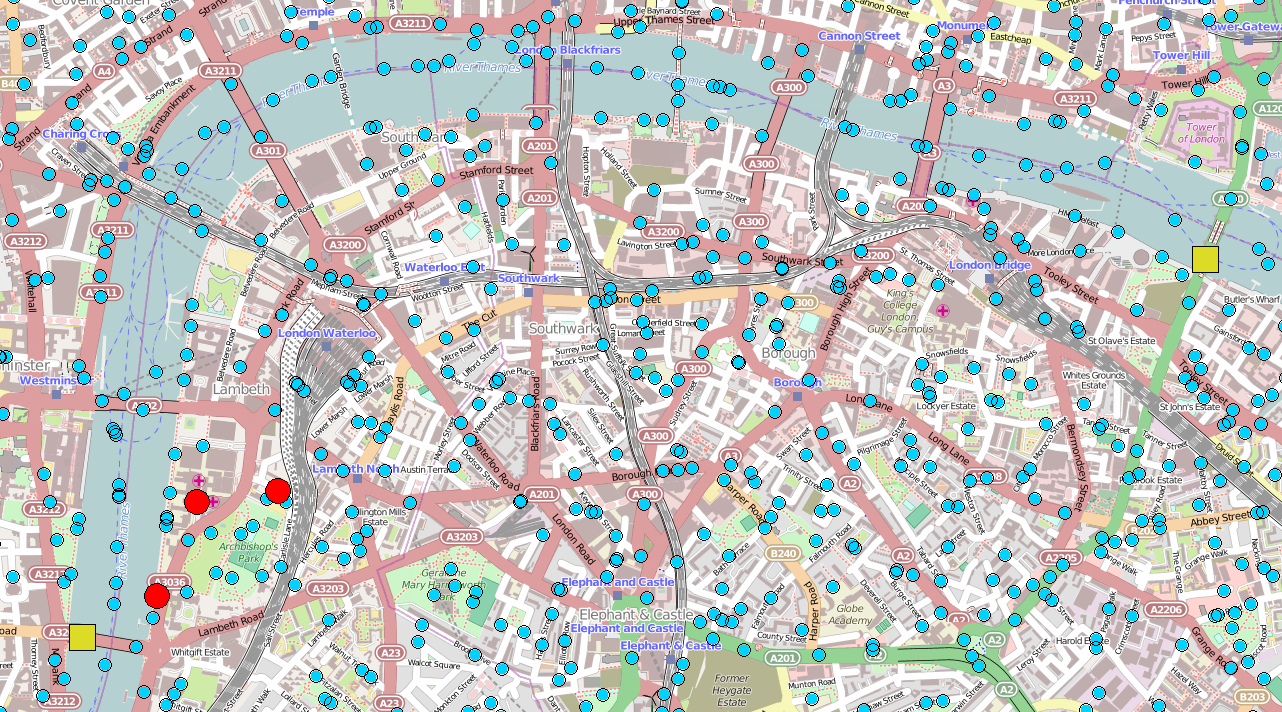
\includegraphics[width=\textwidth{}]{imgs/screenshots/london1}
\end{frame}

\begin{frame}{Rendezvous at a Mass Event}
  \centering
  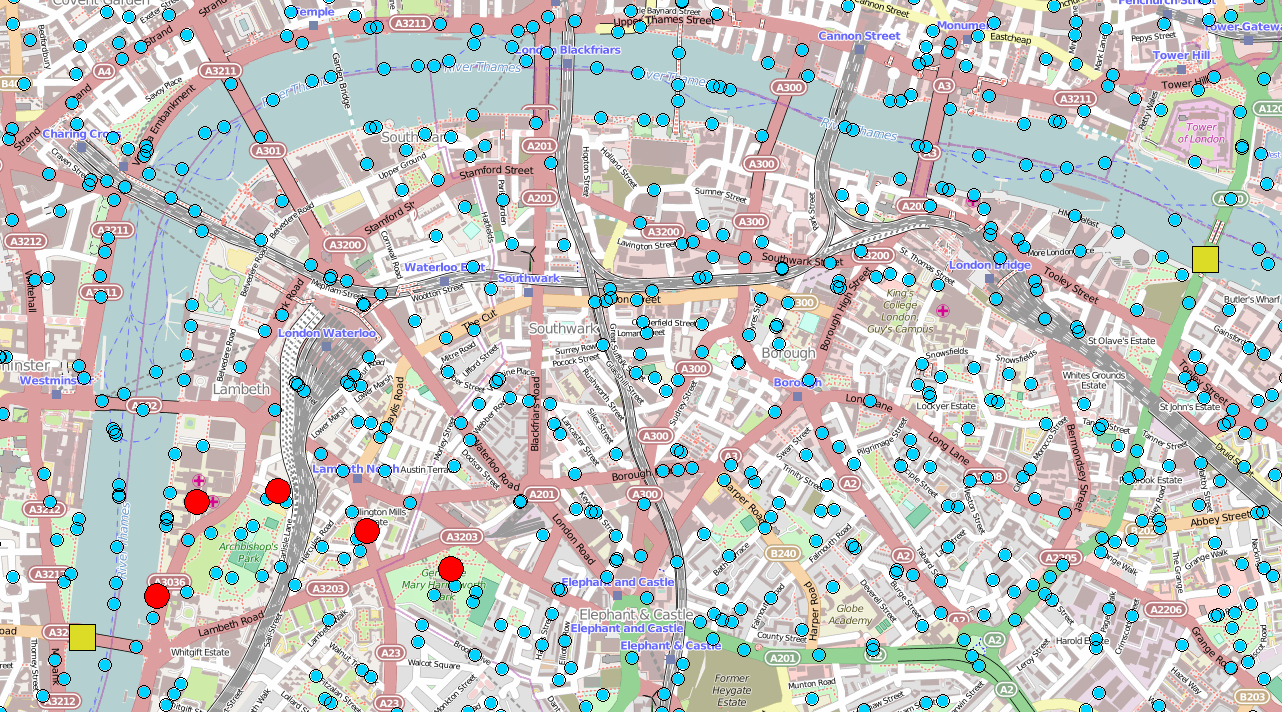
\includegraphics[width=\textwidth{}]{imgs/screenshots/london2}
\end{frame}

\begin{frame}{Rendezvous at a Mass Event}
  \centering
  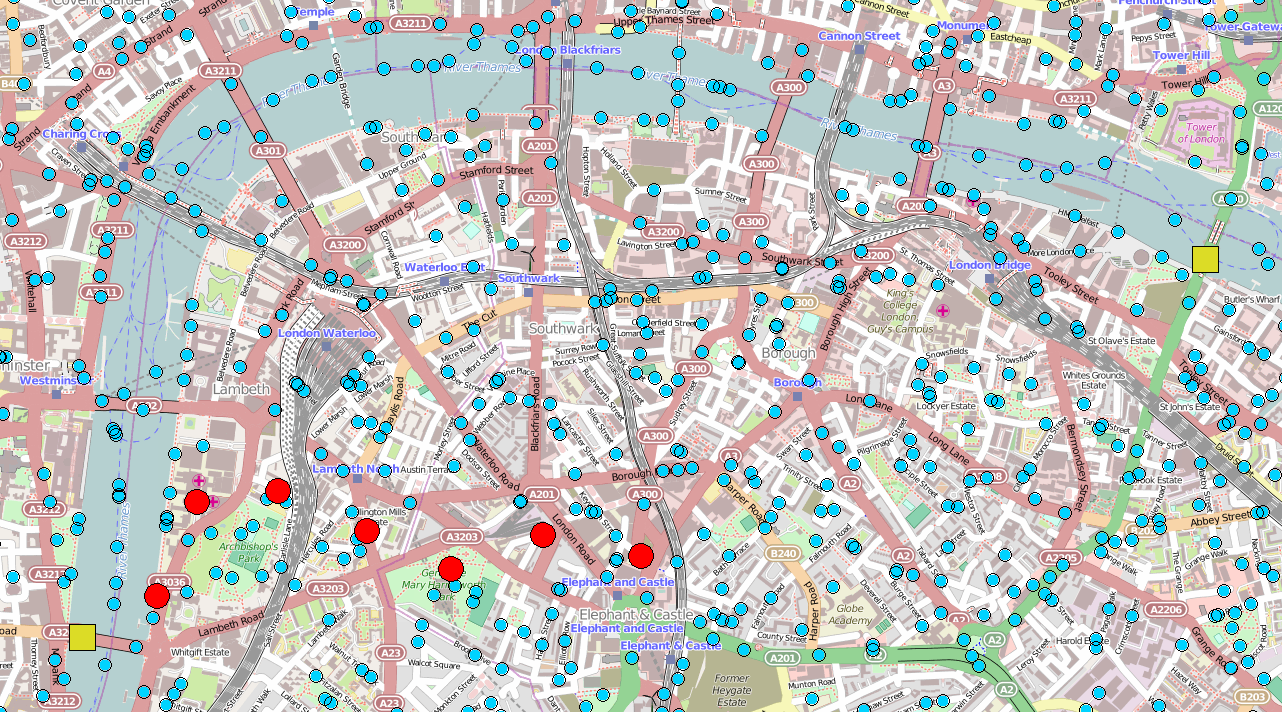
\includegraphics[width=\textwidth{}]{imgs/screenshots/london3}
\end{frame}

\begin{frame}{Rendezvous at a Mass Event}
  \centering
  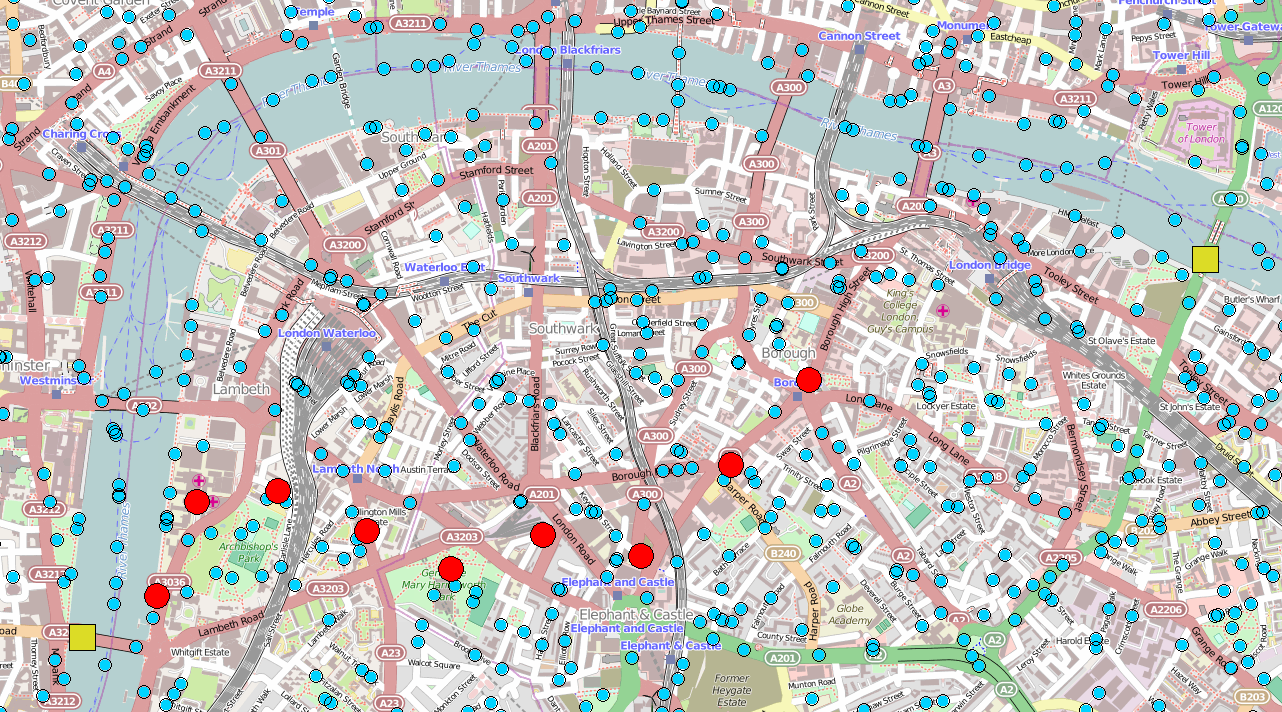
\includegraphics[width=\textwidth{}]{imgs/screenshots/london4}
\end{frame}

\begin{frame}{Rendezvous at a Mass Event}
  \centering
  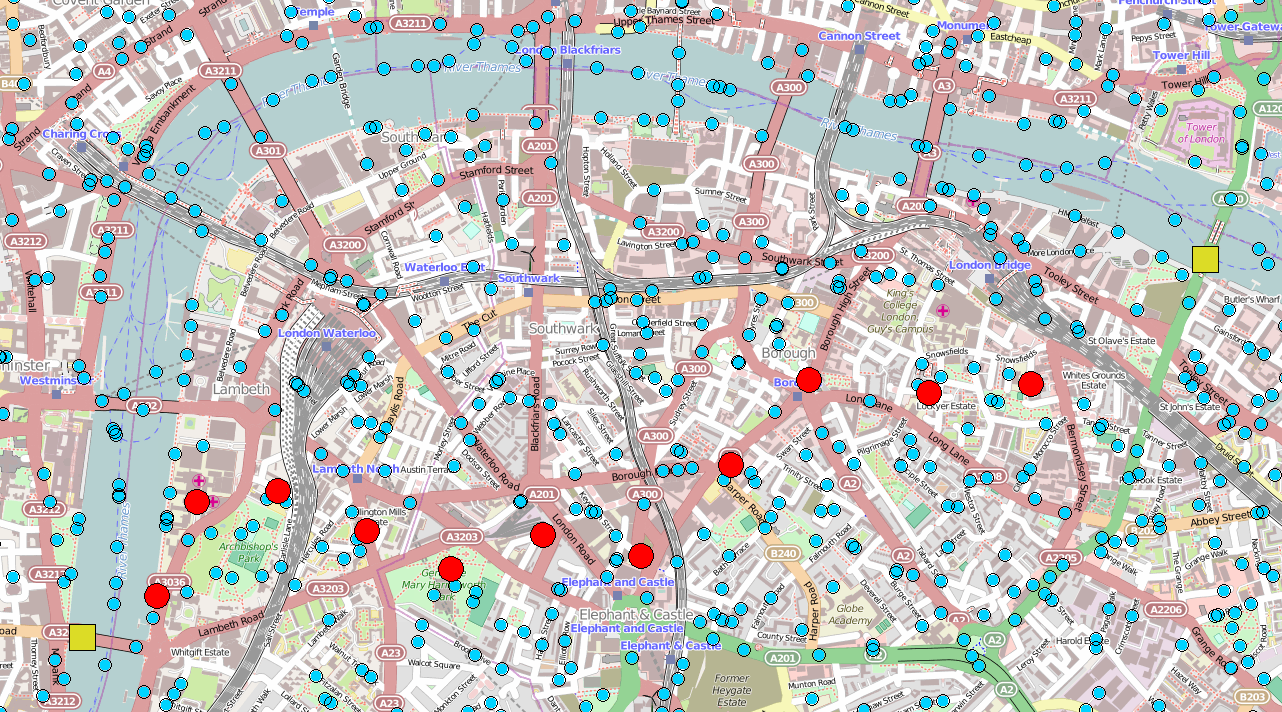
\includegraphics[width=\textwidth{}]{imgs/screenshots/london5}
\end{frame}

\begin{frame}{Rendezvous at a Mass Event}
  \centering
  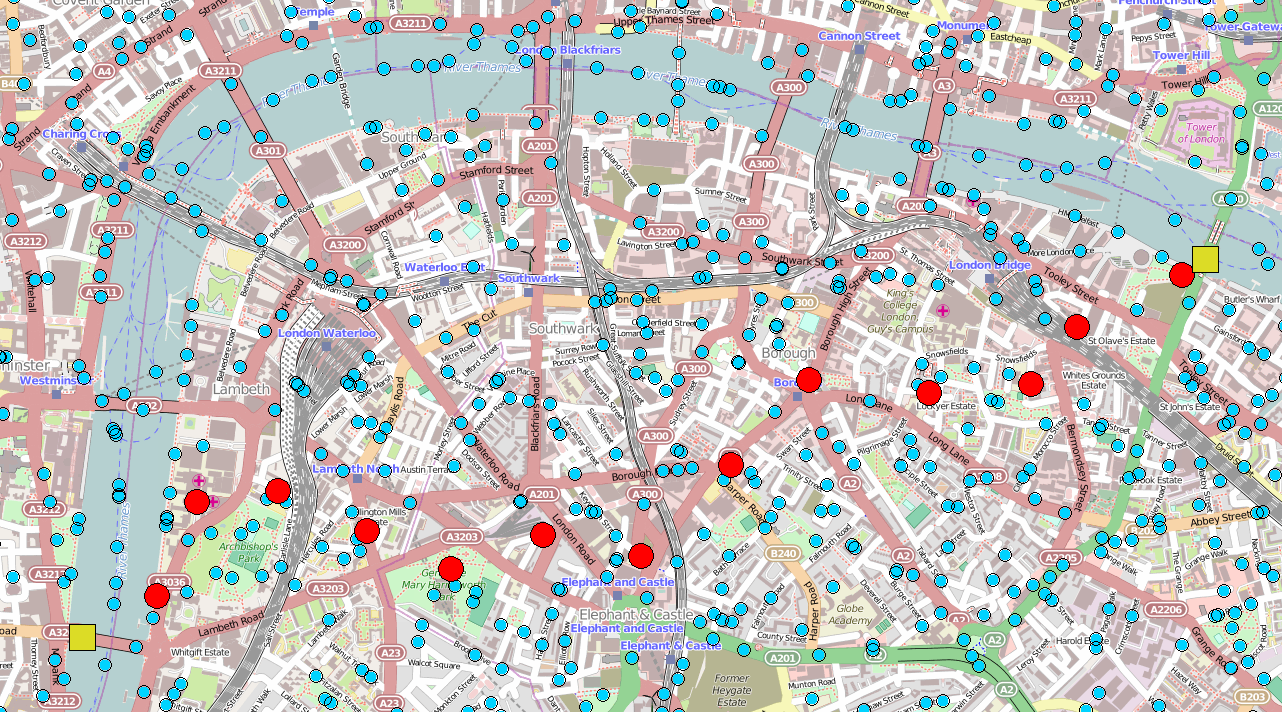
\includegraphics[width=\textwidth{}]{imgs/screenshots/london6}
\end{frame}

\begin{frame}{Network Service Management}
  \begin{block} {Problem}
   \begin{itemize}
    \item Legacy or poorly coded services do not respond gracefully to the failure of their dependencies
    \item Risk of inconsistent state and of being unable to resume correctly when the failed dependency is back online
   \end{itemize}
  \end{block}
  \begin{block} {Possible solution with Protelis}
   \begin{itemize}
    \item Attach a Protelis daemon to each service, which watches its status and communicates with other daemons to coordinate shutdown and restart
   \end{itemize}
  \end{block}
  \begin{block} {Testbed}
   \begin{itemize}
    \item Implemented on a network of EmuLab servers
    \item Services are emulated by query-response networking Java programs
    \begin{itemize}
      \item they ``hang'' when triggered or when their queries consistently fail
    \end{itemize}
   \end{itemize}
  \end{block}
\end{frame}

\begin{frame}{Network Service Management}
  \centering
  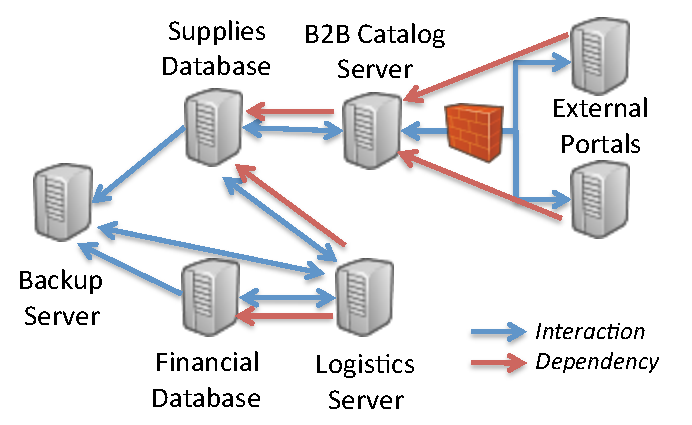
\includegraphics[width=\textwidth{}]{imgs/managementScenario}
\end{frame}

\begin{frame}[fragile]{Network Service Management}
\begin{Verbatim}[fontsize=\scriptsize, frame=none, commandchars=\\\{\}]
\km{import} it.unibo.alchemist.language.protelis.datatype.Tuple.*
\km{import} com.bbn.a3.distributedrestart.DaemonNode.*

\il{Compare required and available services}
\km{let} \vb{nbr_set} = \fc{unionHood}(\fc{nbr}([\ex{serviceID}]));
\km{let} \vb{nbr_missing} = \ex{dependencies}.\ex{subtract}(\vb{nbr_set});
\km{let} \vb{nbr_required} = \ex{#contains}(\ex{dependencies}, \fc{nbr}(\ex{serviceID})); 
\km{let} \vb{nbr_down} = \fc{nbr}(\ex{managedServiceStatus}==\str{"hung"} || \ex{managedServiceStatus}==\str{"stop"});

\il{Is service currently safe to run?}
\km{let} \vb{problem} = \fc{anyHood}(\vb{nbr_down} && \vb{nbr_required}) || !\vb{nbr_missing}.\ex{isEmpty}();

\il{Take managed service up and down accordingly}
\fc{if} (\ex{managedServiceStatus} == \str{"run"} && \vb{problem}) \{
  \ex{#stopProcess}(\ex{managedService});
\} \fc{else} \{
  \fc{if} (\ex{managedServiceStatus}==\str{"stop"} && !\vb{problem}) \{
    \ex{#startProcess}(\ex{managedService});
  \} \fc{else} \{
    \ex{managedServiceStatus}
  \}
\}
\end{Verbatim}
\end{frame}

\begin{frame}{Network Service Management}
  \centering
  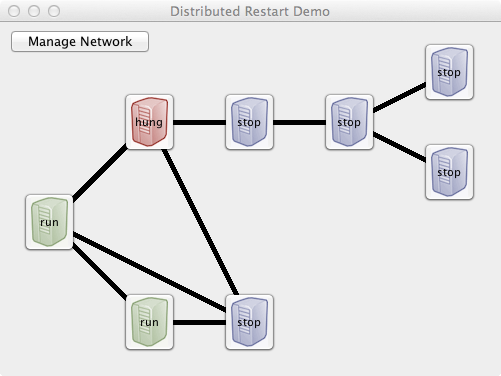
\includegraphics[width=0.8\textwidth{}]{imgs/management}
\end{frame}

\section{Conclusion and Future work}

\begin{frame}{Conclusion and Future Work}
  \begin{block} {Conclusion}
   \begin{itemize}
    \item Universality and coherence by building atop the field calculus
    \item Accessibility, portability and ease of integration by Java interoperability
    \item Important component of the toolchain necessary for using aggregate programming in practice
   \end{itemize}
  \end{block}
  \begin{block} {Future work}
   \begin{itemize}
    \item Development is very active
    \item Next step: use Protelis to build a library of reusable, high-level building blocks for distributed applications.
   \end{itemize}
  \end{block}
\end{frame}





%===============================================================================
\section*{\refname}
%===============================================================================
\begin{frame}[allowframebreaks]
%\begin{frame}[t,allowframebreaks]
  \frametitle{\refname}
  \scriptsize
  \bibliographystyle{alpha}
  \bibliography{bibliography}
\end{frame}
\section*{\refname}
%===============================================================================

\againframe{coverpage}

\begin{frame}[fragile]{Simpler semantics}
  \begin{columns}
    \begin{column}{6cm}
      \centering
      Proto \\
      \begin{framed}
        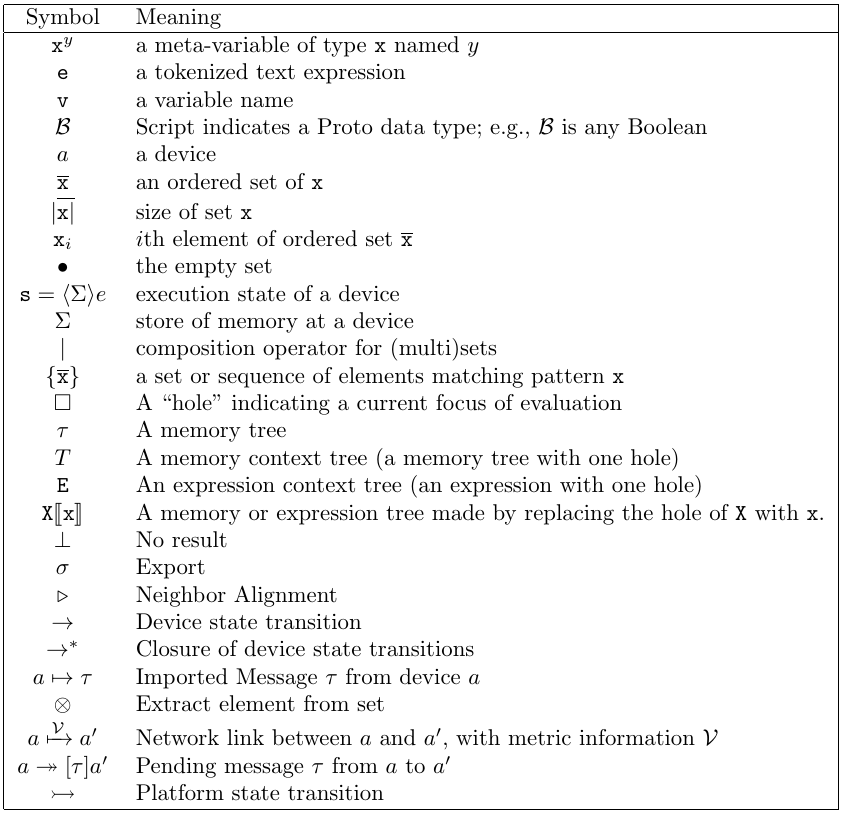
\includegraphics[width=0.31\columnwidth]{imgs/protosem1} 
        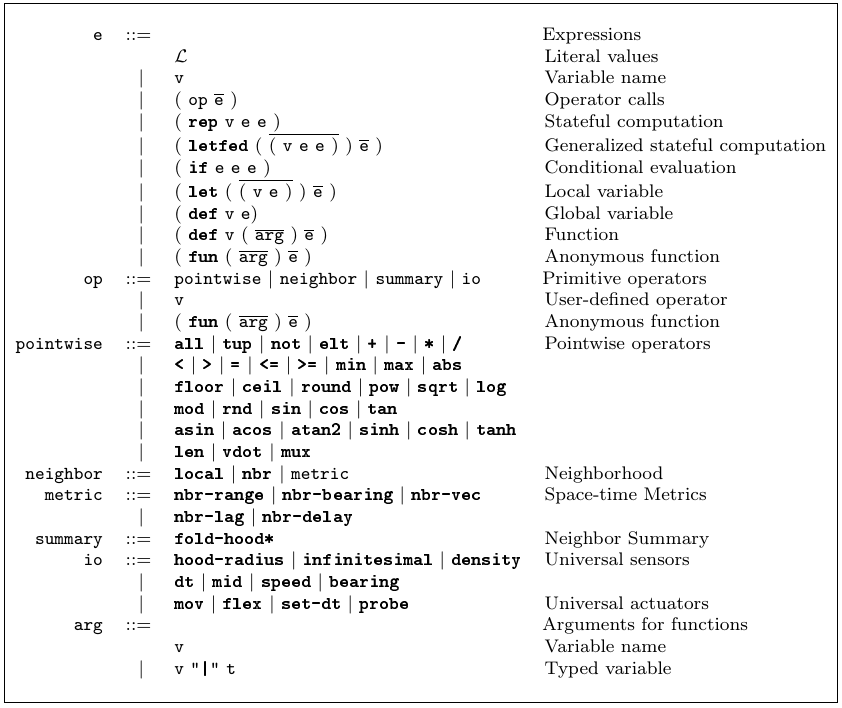
\includegraphics[width=0.35\columnwidth]{imgs/protosem2} \\
        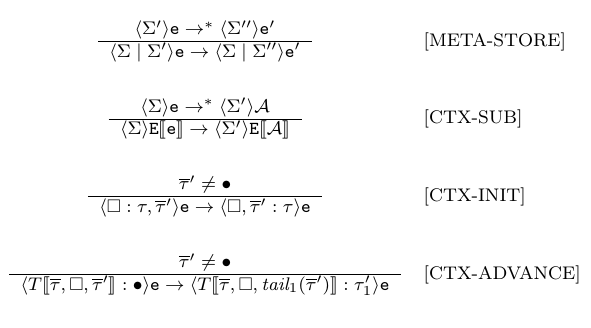
\includegraphics[width=0.30\columnwidth]{imgs/protosem10} 
        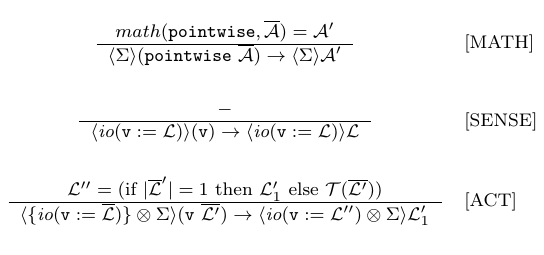
\includegraphics[width=0.37\columnwidth]{imgs/protosem11}
        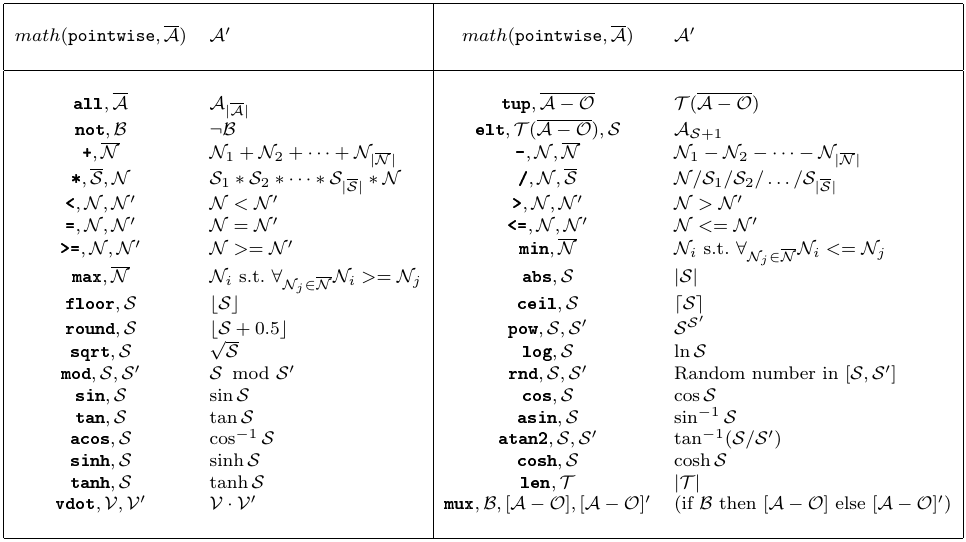
\includegraphics[width=0.30\columnwidth]{imgs/protosem12} \\
        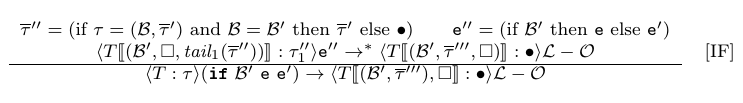
\includegraphics[width=0.40\columnwidth]{imgs/protosem14} \\
        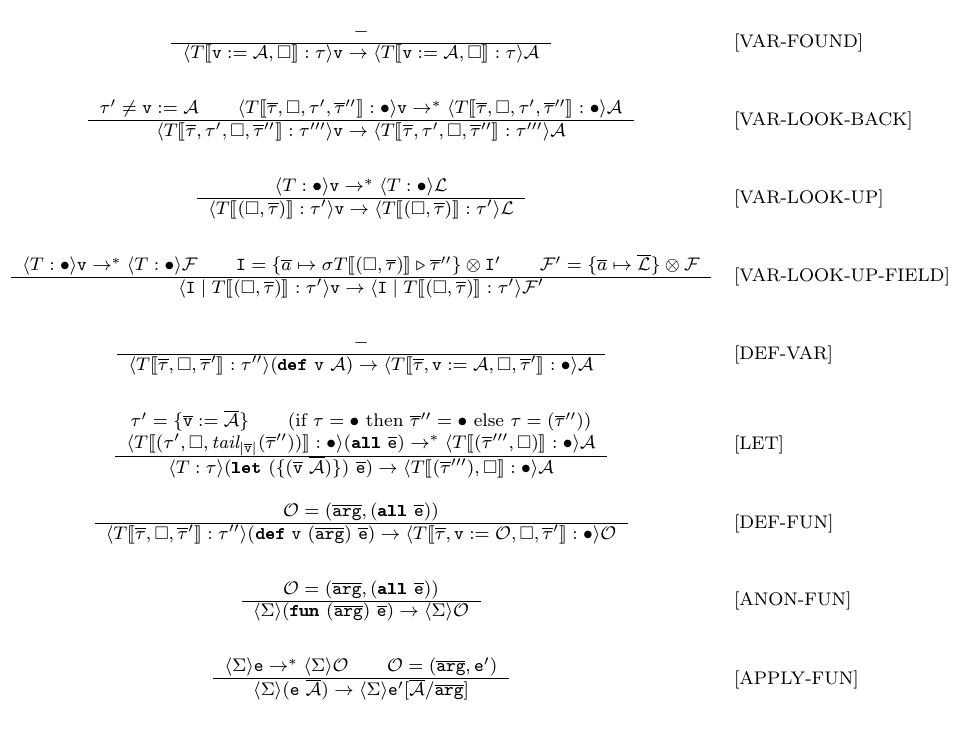
\includegraphics[width=0.39\columnwidth]{imgs/protosem13} 
        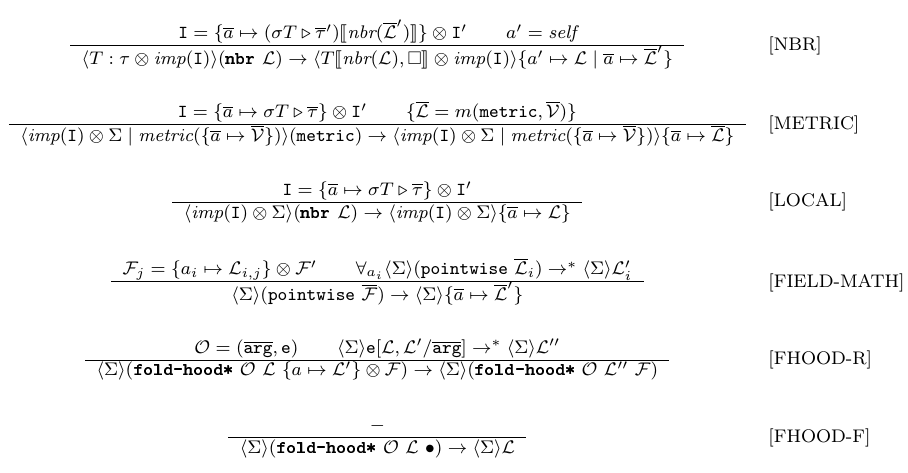
\includegraphics[width=0.59\columnwidth]{imgs/protosem16} \\
        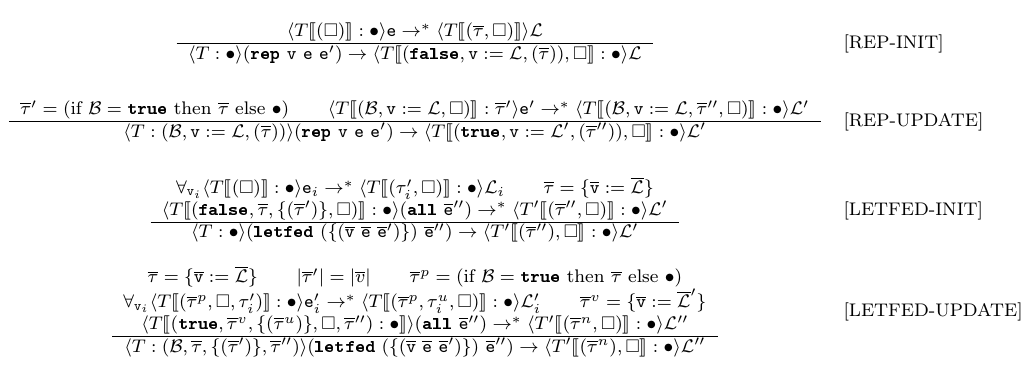
\includegraphics[width=0.49\columnwidth]{imgs/protosem15} 
        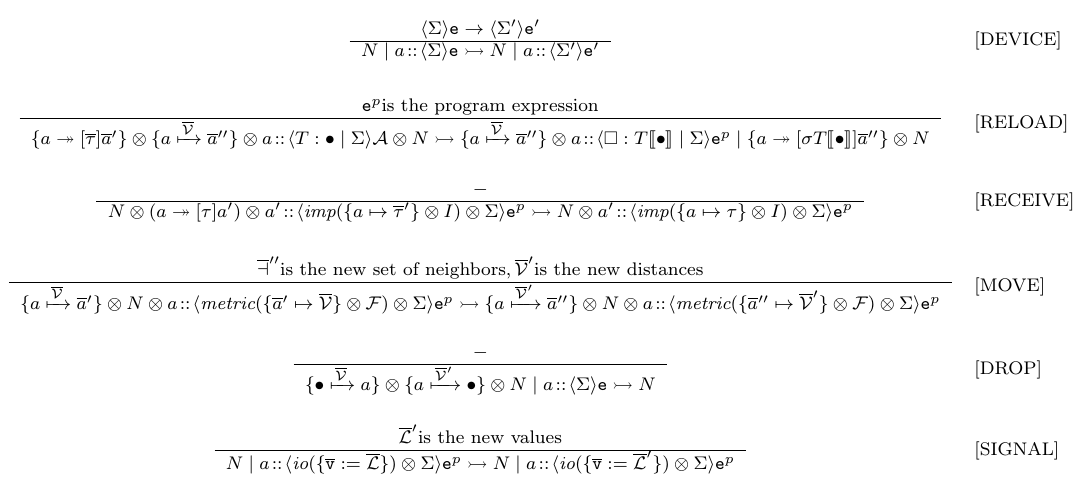
\includegraphics[width=0.49\columnwidth]{imgs/protosem17} 
      \end{framed}
    \end{column}
    \begin{column}{6cm}
      \centering
      Field calculus \\
      \begin{framed}
        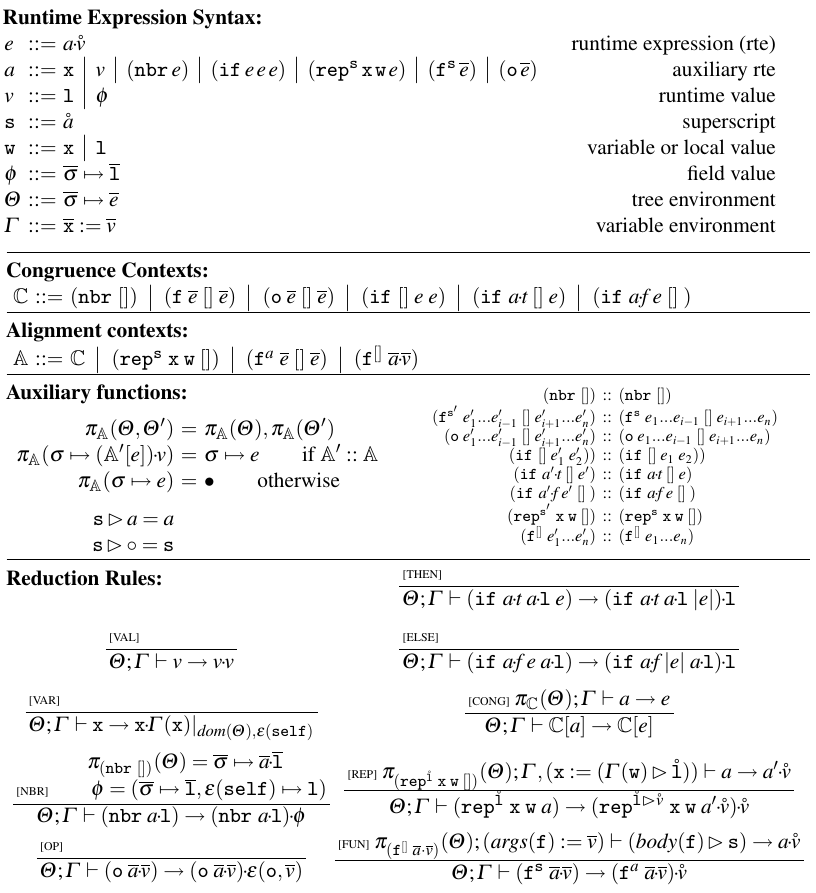
\includegraphics[width=1.015\columnwidth]{imgs/fcsem}
      \end{framed}
   \end{column}
  \end{columns}
\end{frame}



\end{document}
